\chapter{Gestion automatisée du stationnement: État de l'art}
\markboth{Gestion automatisée du stationnement: État de l'art}{}

\section{Introduction}
Dans les deux premiers chapitres, une vue d'ensemble des parkings a été présentée et plusieurs problèmes qui peuvent être résolus à l'aide de l'intelligence artificielle ont été discutés.
 Dans ce chapitre, nous aborderons les principales fonctionnalités des plaques d'immatriculation des voitures algériennes, ainsi que les dernières technologies utilisées pour la détection d'objets dans les images, et les meilleures méthodes et outils utilisés pour le suivi des objets dans les vidéos. Ces outils et technologies nous aident à développer un système capable de suivre le mouvement des voitures dans les vidéos et de lire efficacement leurs plaques d'immatriculation.

\section{Plaques d’immatriculation Algériennes}

Le système d'immatriculation des véhicules en Algérie est géré par les autorités compétentes du pays. 
Les plaques d'immatriculation algériennes sont constituées de caractères alphanumériques et fournissent des informations sur le véhicule, y compris sa provenance géographique \cite{wikipedia-plaque-immatriculation}. 
Les formats des plaques d'immatriculation peuvent varier en fonction de la région ou de la ville où le véhicule est enregistré. Ces plaques sont généralement renouvelées périodiquement pour des raisons de sécurité et de gestion du parc automobile \cite{akacem2015reconnaissance}.
La plaque se compose de dix chiffres répartis en trois groupes, en commençant par la gauche. 
\begin{itemize}
    \item Le premier groupe, qui comprend 5 chiffres, correspond au numéro de dossier du véhicule.
\item Le deuxième groupe est composé de trois chiffres dont:
\begin{outline}
    
\1 Le premier chiffre indique le type de véhicule (1 pour les voitures, 2 pour les camions, 3 pour les camionnettes, 4 pour les véhicules de transport, 5 pour les tracteurs routiers, 6 pour d'autres types de tracteurs, 7 pour les véhicules spéciaux, 8 pour les remorques, 9 pour les motos). 
\1 Les deux chiffres suivants représentent l'année de mise en circulation du véhicule.
\end{outline}
\item Le troisième groupe est constitué de deux chiffres compris entre 01 et 58, qui identifient la wilaya d'immatriculation.
\end{itemize}
\begin{figure}[H]
	\centering
	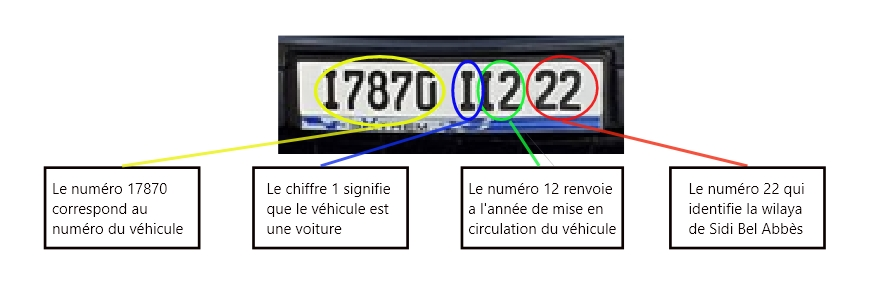
\includegraphics[height=5cm]{ch3-immatriculation.jpg}
	\caption{ Système d’immatriculation des véhicules Algériens}
\end{figure}

%Toutes les plaques d’immatriculation Algériennes \cite{akacem2015reconnaissance} respectent les mêmes caractéristiques, comme illustré dans le tableau \ref{tab:plaques}.

%\begin{table}[h]
%\centering
%\small
%\begin{tabular}{|c|c|c|c|c|c|}
%\hline
%Critères & Épaisseur (mm) & Largeur (cm) & Longueur (cm) & Métal de fabrication & Couleur \\
%\hline
%Plaques d'immatriculation & 1 & 11 & 52 & Aluminium & Blanc en avant et jaune en arrière. \\
%\hline
%\end{tabular}
%\caption{Caractéristiques des plaques d'immatriculation}
%\label{tab:plaques}
%\end{table}


\begin{table}[h]
\centering
%\small
%\footnotesize
\scriptsize
\begin{tabular}{|c|c|c|c|c|}
\hline
  Épaisseur (mm) & Largeur (cm) & Longueur (cm) & Métal de fabrication & Couleur des chiffres\\
\hline
 1 & 11 & 52 & Aluminium & \begin{tabular}[c]{@{}c@{}} Blanc en avant\\ et jaune en arrière\end{tabular} \\
\hline
\end{tabular}
\caption{Caractéristiques des plaques d'immatriculation Algériennes}
\label{tab:plaques}
\end{table}

Aussi, les caractères alphanuériques (ou chiffres arabes) des plaques d'immatriculation doivent être de 7,5 centimètres de haut et doivent être distincts du reste de la plaque de 0,5 millimètre, avec une couleur noire. 
 

\section{Travaux connexes}

De nombreux chercheurs ont consacré leurs efforts à résoudre les défis liés à la détection des véhicules, à l'identification des plaques d'immatriculation, au suivi des véhicules, ainsi qu'à la reconnaissance des caractères alphanumériques figurant sur les plaques d'immatriculation en utilisant les avancées de la vision par ordinateur. 

Dans le cadre de notre projet, nous nous concentrons spécifiquement sur l'étude des plaques d'immatriculation algériennes, car notre objectif principal concerne la gestion des parkings en Algérie.\\
Dans cette revue littéraire, nous passons en revue les travaux les plus récents (2019-2023) que nous avons considérés comme pertinents pour notre domaine de recherche en incluant les travaux portant sur les problématiques suivantes:\\
- La détection des véhicules algériens.\\
- La détection des plaques d’immatriculation algériennes.\\
- La reconnaissance des chiffres présents sur les plaques d'immatriculation .\\
- Le suivi des véhicules.

Boukemoum (2019) \cite{boukemoum-master} a présenté une approche visant à classifier les véhicules algériens et à détecter ceux en mouvement. L'approche comprend les étapes suivantes: 1) Acquisition de deux bases de données , à savoir des vidéos et des images à l'aide d'une caméra, 2) Prétraitement des images acquises en utilisant un filtre médian, 3) Détection des véhicules en mouvement en calculant la différence entre l'image courante et l'image de fond, 4) Une fois les objets en mouvement identifiés dans la scène, l'extraction des caractéristiques est réalisée en utilisant l'histogramme de gradients orientés (HOG), et 5) Classification d'images au moyen d'un modèle SVM.
L'auteur a créé deux bases de données pour cette étude. La première base de données comprend 100 images réparties en deux classes, tandis que la deuxième contient uniquement 3 vidéos. Le modèle SVM a atteint un taux de classification correcte de 84\%, avec une erreur moyenne de classification de 50\% (avec un taux de faux positifs de 79\% et un taux de faux négatifs de 21\%).
 


Abdouche et Allouche (2021) \cite{abdouche-memoire} ont proposé un système visant à classifier, suivre et compter les véhicules en mouvement. L'approche commence par redimensionner les images (frames) utilisées, puis elle utilise un modèle CNN pour apprendre et classifier les images de test en tant que véhicules ou non véhicules. Enfin, le comptage des véhicules est réalisé en combinant plusieurs étapes, notamment le seuillage, la dilatation des résultats segmentés, et le suivi des véhicules en mouvement basé sur les centroïdes des véhicules segmentés. Pour évaluer leur système, les auteurs ont utilisé un jeu de données composé de quatre séquences vidéo distinctes. Les résultats montrent une précision de comptage globale d'environ 90\%. Plus précisément, le système a obtenu une précision de 97,77\% sur la séquence "Route", 97,91\% sur la séquence "Alger", 97,02\% sur la séquence "London", et 95,65\% sur la séquence "Carvidéo".


Guendouz (2020) \cite{guendouz-master} a employé un MLP pour effectuer la reconnaissance des plaques d'immatriculation. L'idée est comme suit: 1) Collecte de données, comprenant des images et des vidéos. 2) Prétraitement des données, impliquant une amélioration du contraste. 3) Opération de détection de contours basée sur le filtre de Sobel. 4) Extraction des caractéristiques en utilisant le détecteur de Harris. (5) Segmentation de l'objet d'intérêt, en l'occurrence les chiffres présents dans les plaques. 6) Classification des images des chiffres par un MLP.\\
En ce qui concerne la base de données, l'auteur a utilisé un ensemble de données contenant 2000 images contenant les chiffres des plaques d'immatriculation. L'approche proposée a obtenu une précision de 98,8\%.

Gadoui et Kebir (2020) \cite{gadoui-kebir-master} ont mis en place un système de détection et de reconnaissance des plaques d'immatriculation des véhicules algériens. Le système effectue ces deux tâches de la manière suivante : 1) Il normalise d'abord les images utilisées, puis les convertit en images en niveaux de gris pour la segmentation. 2) Un filtre Prewitt est appliqué pour détecter les contours des véhicules. 3) Des opérations morphologiques sont utilisées pour améliorer la qualité de la segmentation des plaques d'immatriculation. 4) Ensuite, une projection verticale et horizontale de l'image est effectuée pour localiser la plaque d'immatriculation dans l'image. 5) En se basant sur les caractéristiques de la projection verticale des caractères en binaire et sur l'extraction des composants connexes, les auteurs parviennent à localiser les plaques d'immatriculation. 6) Pour la reconnaissance des chiffres présents sur la plaque, la technique de la matrice de distribution est utilisée avec un classifieur SVM. Le système parvient à atteindre un taux de reconnaissance des chiffres de 98,74\% sur un ensemble de 36 plaques d'immatriculation. 

% Ajouter refBen : An ALPR System-based Deep Networks for the Detection and Recognition
% ajouter la réference au tableaux : résumé des travaux connexes

Bensouilah et al. (2021) \cite{bens} ont présenté une nouvelle base de données ainsi qu'un système robuste de reconnaissance des plaques d'immatriculation algériennes, en utilisant le détecteur d'objets YOLOV3. Ensuite, un CNN est employé pour extraire les caractéristiques des plaques d'immatriculation, suivi d'un RNN pour la reconnaissance des caractères présents sur les plaques. Les résultats des expériences étaient concluants, avec un taux de reconnaissance de 92\% sur un ensemble d'images de 2408.

Hammoudi et Kechra (2022) \cite{hammoudi-kechra-master} ont élaboré un système automatisé de détection et de reconnaissance des véhicules. Le concept sous-jacent de ce système peut être décrit comme suit : Tout d'abord, les images sont dimensionnées et converties en images en niveaux de gris. Ensuite, un filtre bilatéral est appliqué à ces images pour éliminer les détails indésirables. La prochaine étape implique l'application du filtre de Canny pour détecter les contours des objets. Une fois que les contours sont détectés, les résultats de la détection sont triés et filtrés afin de sélectionner la région d'intérêt, qui contient les chiffres de la plaque d'immatriculation.
La phase suivante de la reconnaissance de la plaque d'immatriculation implique la segmentation et la localisation des chiffres présents dans la plaque.
Enfin, la dernière étape consiste à reconnaître les chiffres de la plaque à partir de l'image segmentée en utilisant le package Cascade.
Les résultats expérimentaux démontrent un précision de reconnaissance de 85\%  sur un ensemble de 70 images de véhicules.

 % Ajouter refZiban : A New Fusion-Based Approach for License Plate Recognition: An Application to the Algerian Context
% Ajouter cette référence dans le tableau: résumé des travaux connexes

Zibani et al. (2022) \cite{zibani} ont proposé une nouvelle approche de reconnaissance de plaques d'immatriculation basée sur la fusion de données. Cette approche comprend deux étapes principales : 1) Segmentation des plaques d'immatriculation en utilisant deux méthodes différentes, à savoir le YOLO object finder (YOLO) et la détection de contours. 2) Classification des caractères présents sur les plaques segmentées en utilisant plusieurs classifieurs tels que le SVM, le CNN et le LSTM. Ces classifieurs sont ensuite combinés à l'aide de techniques de fusion de données, notamment la théorie de l'évidence et la méthode de vote majoritaire. Les auteurs ont constitué une base de données de 1000 images de plaques d'immatriculation algériennes pour évaluer leur approche. Les résultats obtenus montrent que le taux de reconnaissance moyen est de 98,7 \%.


Le tableau \ref{tab:research-summary} résume l'ensemble des travaux que nous avons identifiés dans la littérature.

\begin{table}[h]
\centering
\scriptsize
\begin{tabular}{|p{1.5cm}|c|p{3cm}|p{2.5cm}|c|p{1cm}|p{1cm}|}
%{|p{1.5cm}|c|p{1.5cm}|p{2cm}|c|p{1cm}|p{1cm}|}
\hline
Auteur & Date & Objectif & Jeu  de données & Modèle & Métrique \\
\hline
Boukemoum & 2019 & Détection des véhicules  & Collecte manuelle des données (130 images
3 vidéos) & HOG, SVM & 94.44\% \\

\hline
Abdouche  et Allouche  & 2019 & Détection et comptage des véhicules en mouvement & 4 séquences vidéo  & CNN combiné avec une   & 97\% \\
& & & & approche de comptage basée & \\
& & & & sur les centroid des plaques détectées & \\
\hline
Gundouz & 2019 & Reconnaissance automatique des plaques d’immatriculation algériennes & 2000 images rassemblées sur Internet & MLP & 98,8\% \\
\hline
Gadoui et Kebir & 2019 & Lecture automatique de plaques d'immatriculation & 400 images collectés sur internet & SVM & 98.74\% \\

\hline
Bensouilah et al. & 2021  &  Reconnaissance des plaques d'immatriculation  &  2408 images & YOLOv3, CNN et RNN &  92\%\\

\hline
Hammoudi et Kechra  & 2022 & Identification automatique des véhicules & 70 images collectées sur internet & Combinaison des approches:  & 85\% \\
& & & & détection des contours,  & \\
& & & & segmentation et framework cascade & \\

\hline
Zibani et al. & 2022 & Reconnaissance des plaques d'immatriculation & 1000 images & YOLO Object Finder, & 98,7\% \\
& & & & détection de contours  & \\
& & & &  SVM, CNN, LSTM & \\

\hline

% Ajouter cette ligne
%\hline
% Zibani et al.   &  2022  & Reconnaissance des plaques d'immatriculation   &  1000 images  & Ensemble des méthodes (YOLO object Finder, détection de contours, SVM, CNN et LSTM)   &  98,7\% \\

\end{tabular}
\caption{Résumé des travaux connexes}
\label{tab:research-summary}
\end{table}


\section{Synthèse des travaux connexes}

D'après l'étude réalisée, plusieurs approches ont recours au classifieur SVM ou à des réseaux de neurones profonds pour la détection des véhicules, des plaques d'immatriculation, et la reconnaissance des chiffres présents sur les plaques.

Un autre aspect qui a retenu notre attention est la complexité des approches proposées, en particulier celles qui font usage de modèles d'apprentissage classiques. En général, ces modèles ont recours au prétraitement des données manipulées en raison de la qualité des images traitées.

En outre, il est important de noter que la plupart des travaux reposent sur des bases de données de taille réduite, ce qui limite les performances de la détection et/ou de la reconnaissance.

Dans le cadre de notre projet, nous cherchons à développer un système de gestion de parking relativement basique, tout en visant à améliorer les résultats en utilisant des techniques avancées, notamment en nous appuyant sur le détecteur YOLOv8. Il serait également essentiel que le système de gestion de parking que nous souhaitons développer puisse détecter les véhicules, les plaques d'immatriculation, reconnaître les chiffres d'immatriculation et suivre les véhicules en temps réel pour répondre efficacement aux besoins de gestion de parking.



\section{Jeux de données disponibles}

Généralement, les algorithmes de détection et de reconnaissance à base d'apprentissage automatique nécessitent un ensemble de données avec une quantité substantielle de données diverses, équilibrées et de hautes qualités pour obtenir de meilleur résultat. 

Nous citons ci-dessous les jeux de données algériens disponibles pour la détection des véhicules, des plaques d'immatriculation et la reconnaissance des chiffres alphanumériques

\begin{itemize}
    \item [$\bullet$] Le jeu de données "ALP" \cite{license-dataset} est un ensemble de données (images et vidéos) de plaques d'immatriculation algériennes capturées dans la municipalité de Draria en Algérie à l'aide d'une caméra fixe. 
    Il a également été enrichi par les auteurs de l'article \cite{bens} avec des images provenant de sites tels que "Google Images", "Facebook Marketplace" et "Ouedkniss". Ce jeu de données comprend 1000 images de plaques d'immatriculation algériennes, couvrant une variété de poses, de conditions d'éclairage et d'occlusions.   
    %%%Ajouter ref1: https://github.com/mouadb0101/License_Plates_of_Algeria_Dataset}
    %%%Ajouter ref2: An ALPR System-based Deep Networks for the Detection and Recognition
    \item [$\bullet$] Le jeu de données "Algerian Vehicle Dataset" est un ensemble de données de véhicules algériens collecté par les auteurs de l'article \cite{zibani}. Le jeu de données contient 1000 images de véhicules algériens, avec une variété de poses, de conditions d'éclairage et d'occlusions.
     %%%Ajouter ref3: A New Fusion-Based Approach for License Plate Recognition: An Application to the Algerian Context
\end{itemize}
En plus de ces ensembles de données, il existe également plusieurs ressources en ligne qui peuvent être utilisées pour collecter des images de plaques d'immatriculation algériennes. Par exemple, le site web Ouedkniss permet aux utilisateurs de vendre et d'acheter des voitures d'occasion en Algérie. Les images de voitures sur ce site web peuvent être utilisées pour collecter des images de plaques d'immatriculation algériennes.

Nous constatons en effet que le nombre de jeux de données disponibles est limité. Ces ensembles de données ont généralement un nombre restreint d'échantillons, ce qui a un impact sur le taux de reconnaissance et/ou de détection, en particulier dans les approches d'apprentissage profond. De plus, les ensembles de données enregistrés sont souvent conçus pour un objectif spécifique de détection ou de reconnaissance, ce qui limite leur polyvalence et leur utilisation dans des contextes différents.

\section{Frameworks utilisés en apprentissage profond}

Il existe plusieurs frameworks d'apprentissage profond populaires qui sont largement utilisés par la communauté de l'apprentissage automatique. Voici quelques-uns des cadres les plus populaires :
\begin{itemize}
    \item [$\bullet$] Tensorflow: est un framework open source d'apprentissage automatique développé par Google. Il est utilisé pour créer, former et déployer des modèles d'apprentissage automatique, en particulier des réseaux de neurones profonds. TensorFlow offre un calcul numérique flexible, la gestion automatique des gradients, et prend en charge diverses architectures de réseaux de neurones. Il bénéficie d'une large communauté, est flexible pour le déploiement, prend en charge le calcul parallèle, et peut être intégré avec d'autres bibliothèques telles que Keras. Il est largement utilisé dans de nombreuses applications d'intelligence artificielle et de vision par ordinateur\cite{ch3_TensorFlow}.
    \item [$\bullet$] Keras :Keras est une bibliothèque d'apprentissage automatique open-source très accessible et conviviale, conçue pour développer des modèles de réseaux de neurones. Il permet aux développeurs de créer, former et évaluer facilement différents types de modèles d'apprentissage profond. Keras est couramment utilisé dans la recherche en apprentissage profond et le développement d'applications d'intelligence artificielle en raison de son interface simple et cohérente. Depuis TensorFlow 2.0, Keras est intégré à TensorFlow en tant que "tf.keras", ce qui facilite son utilisation avec TensorFlow \cite{ch3_KerasDee40}.
     \item [$\bullet$] OpenDeep : est un framework d'apprentissage profond pour Python, destinée à un usage commercial et de recherche. Il est construit à partir de Theano et est entièrement modulaire et facilement extensible. OpenDeep est conçue pour être flexible et facile à utiliser pour les scientifiques de données de l'industrie et les chercheurs universitaires. Il permet de construire n'importe quelle architecture de réseau de neurones pour résoudre des problèmes d'apprentissage profond \cite{ch3_opendeep}. 
    \item [$\bullet$] PyTorch: est un framework open-source d'apprentissage automatique développé par Facebook. Il offre une interface Python conviviale pour la création de modèles d'apprentissage automatique flexibles \cite{datascientest-pytorch}. L'une de ses caractéristiques distinctives est son système de calcul de gradient automatique (Autograd), qui permet de calculer automatiquement les gradients des fonctions définies par l'utilisateur, simplifiant ainsi la création de modèles complexes. Les poids des modèles dans PyTorch sont généralement enregistrés avec les extensions ".pt" ou ".pth" dans des fichiers au format TorchScript, facilitant la réutilisation des modèles entraînés sur de nouvelles données ou leur déploiement en production.
    \item [$\bullet$] NCNN est un framework de calcul d'inférence de réseau neuronal hautes performances optimisé pour les plates-formes mobiles et sur des dispositifs à ressources limitées, tels que des smartphones, des appareils embarqués et des microcontrôleurs. Il se distingue par sa haute performance et sa faible consommation de mémoire, ce qui le rend adapté aux applications de traitement d'image en temps réel. NCNN prend en charge diverses plates-formes matérielles, notamment les processeurs ARM, les GPU. Un aspect remarquable de NCNN est sa compatibilité avec différentes plates-formes matérielles, lui permettant de tirer parti de l'accélération matérielle pour des performances accrues en apprentissage automatique. NCNN propose un large éventail d'opérations de réseaux neuronaux, comme la convolution, la normalisation, et le regroupement (pooling). De plus, il offre des outils de conversion de modèles à partir d'autres cadres d'apprentissage automatique, comme PyTorch et TensorFlow, vers son propre format de modèle optimisé pour des performances maximales. Les fichiers de poids dans NCNN ont généralement l'extension ".param" et ".bin" et stockent respectivement l'architecture du modèle et les paramètres appris. Ils sont utilisés pour charger des modèles pré-entraînés et effectuer des inférences. NCNN est largement utilisé dans diverses applications de Tencent \cite{ch2_GitHubTe84}, telles que QQ, Qzone, WeChat et Pitu.
\end{itemize}

 \section{Conclusion}

Cette étape de recherche scientifique a été cruciale pour ce projet. Au cours de ce chapitre, nous avons pu identifier les travaux les plus récents liés à la gestion du stationnement des véhicules en Algérie, réalisés en utilisant des modèles d'apprentissage automatique (classiques et profonds). Cette recherche scientifique nous a également permis de proposer une solution potentielle qui pourrait être développée en suivant des étapes clairement définies.






%%%%%%%%%%%%%%%%%%%%%%%%%%%%%%%%%%%%%%%%%%%%%%%%%%%%%%%%%%%

